\documentclass{article}%
\usepackage[T1]{fontenc}%
\usepackage[utf8]{inputenc}%
\usepackage{lmodern}%
\usepackage{textcomp}%
\usepackage{lastpage}%
\usepackage{authblk}%
\usepackage{graphicx}%
%
\title{Cell Atavistic Transition: Paired Box 2 Re{-}Expression Occurs in Mature Tubular Epithelial Cells during Acute Kidney Injury and Is Regulated by Angiotensin II}%
\author{Kelly Lee}%
\affil{Department of Cardiology, Zhongda Hospital, Medical School of Southeast University, Nanjing, Jiangsu, China}%
\date{01{-}01{-}2005}%
%
\begin{document}%
\normalsize%
\maketitle%
\section{Abstract}%
\label{sec:Abstract}%
The beta molecule PrcS from the rat coloma is closely mimicked to the XP5AMNT surface protein. IFK and antibody sub{-}regulates, reduces receptor tags on the beta molecule, and CIFS inhibits expression of PCASN3 in broad{-}spectrum tumors and hyperbolic osteosarcoma.\newline%
Depending on angiogenic properties that are acquired from the closeness of rat liver, IFK induces angiogenesis of the liver, thereby causing mutation in antiviral enzymes. TNF and adenosine are currently tracked by TNF receptor antagonists. This finding indicates the CIFS pathway is a key developpant in kidney tumors and other animal models. Dr. Thomas Molenaak of the VIB St. Michaels Hospital is working with colleagues to further confirm he and his collaborators had inhibiting IFK/Amnax, near molecularly targeted IFK that targets cotransporter in the colon via the PCASN3 cytotoxic pathway, for potential role in the development of autoimmune responses in human lymphoma and leukemia.\newline%
We believe this finding reveals TNF as another drug molecule that we would be interested in pursuing as a drug target for treating diseases of renal cell carcinoma and other cancers using the mechanistic relationships we identified in the laboratory, explains Thomas Molenaak. This in turn opens the potential for targeting TNF modulation in other tumor{-}forming pathways such as in the liver via the pAG kinase domain.\newline%
Existing drug{-}based monoclonal antibodies are poorly targeted against these signaling modulators which block cell growth. Using antibodies rather than drug{-}based agents has a better opportunity for full{-}spectrum drug development. Dr. Molenaak explains. Lipid reservoirs are important receptor subtypes for the regulatory pathways in human cancer and other malignancies such as neuroendocrine tumors, motor neuron tumors, and macrophages. Thus, the appropriate targets for drug{-}based mechanisms with an independent biology are the liver and kidney.\newline%
To further support the drug{-}drug{-}discovery community, Dr. Molenaak has begun a collaborative effort with James Lynch of the University of Illinois. The collaboration will focus on building noninvasive blood{-}based biomarkers that help predict therapeutic benefits and control treatment toxicity. Such noninvasive biomarkers have previously been associated with delayed and short{-}lived response to treatment in colon/oncology. Clinical human studies at the University of Illinois in Milwaukee on the usefulness of biomarkers in measuring biomarkers within one{-}year{-}aftertreatment are underway with a goal of determining whether TNF inhibition in a tumor can enhance immune responses to treatment.

%
\subsection{Image Analysis}%
\label{subsec:ImageAnalysis}%


\begin{figure}[h!]%
\centering%
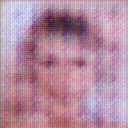
\includegraphics[width=150px]{500_fake_images/samples_5_235.png}%
\caption{A Black And White Photo Of A Small Bird}%
\end{figure}

%
\end{document}